\documentclass{standalone}
\usepackage{tikz}
\begin{document}

    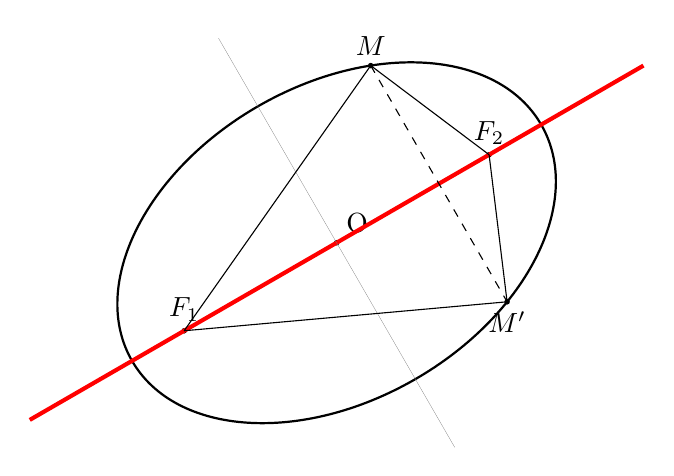
\begin{tikzpicture}[scale = 1]
\def\xC{8}
\def\yC{3}
\def\a{3}
\def\b{2}
\def\ang{30}
% Draw axes
%\draw[->] (-1,0) -- (15,0) node[below] {$x$};
%\draw[->] (0,-1) -- (0,6) node[left] {$y$};

% Ellipse
\draw[thick, rotate around={\ang:(\xC,\yC)}] (\xC,\yC) ellipse [x radius=\a, y radius=\b];

% Center
\fill (\xC,\yC) circle (1pt) node[above right] {O};

% Foci
\pgfmathsetmacro{\c}{sqrt(\a*\a - \b*\b)}
\coordinate (F1) at ({\xC+\c*cos(\ang)},{\yC+\c*sin(\ang)});
\coordinate (F2) at ({\xC-\c*cos(\ang)},{\yC-\c*sin(\ang)});
\fill (F2) circle (1pt) node[above] {$F_1$};
\fill (F1) circle (1pt) node[above] {$F_2$};

\draw [line width =1.5pt, red, rotate around={\ang:(\xC,\yC)}] (3.5,\yC) -- (12.5,\yC);
\draw [line width = 0.1pt, gray, rotate around={\ang:(\xC,\yC)}] (\xC, 0) -- (\xC,6);

\def\theta{60}
\coordinate (M) at
({\xC + \a*cos(\theta)*cos(\ang) - \b*sin(\theta)*sin(\ang)},
 {\yC + \a*cos(\theta)*sin(\ang) + \b*sin(\theta)*cos(\ang)});
\fill (M) circle (1pt) node[above] {$M$};
\coordinate (M') at 
({\xC + \a*cos(360-\theta)*cos(\ang) - \b*sin(360-\theta)*sin(\ang)},
 {\yC + \a*cos(360-\theta)*sin(\ang) + \b*sin(360-\theta)*cos(\ang)});
\fill (M') circle (1pt) node[below] {$M'$};

\draw [-](F1) --(M);
\draw [-](F2) --(M);
\draw [-](F1) --(M');
\draw [-](F2) --(M');
\draw [dashed](M) --(M');

\end{tikzpicture}


\end{document}